\documentclass[11pt, spanish]{article}
\usepackage[spanish]{babel}
\selectlanguage{spanish}
\usepackage[utf8]{inputenc}
\usepackage{graphicx}
\usepackage{mathtools}
\usepackage{tabularx}
\usepackage[font=small,labelfont=bf]{caption}
\usepackage{subcaption}
\usepackage{authblk}
\usepackage{natbib}
\usepackage{multirow}
\usepackage{color}   % For color text: \color command

\captionsetup[table]{name=Tabla}
\renewcommand{\thetable}{\Roman{table}}
\newcommand{\mean}[1]{\left\langle#1\right\rangle}
%\newcommand{\eqref}[1]{Ec.~\ref{#1}}

\graphicspath{
{figuras/},
} % Lugar donde encontrar las figuras generales (se puede poner uno en cada cap{\'{\i}}tulo)

\begin{document}
\begin{titlepage}
    \centering
    {\scshape\LARGE Universidad de Buenos Aires \par}
    \vspace{1cm}
    {\scshape\Large Informe 3:\par}

    \vspace{1.5cm}
    {\scshape\Large\par}
    {\huge\bfseries  Comunidades\par}
    \vspace{2cm}
    {\Large\itshape Ra\'ul Barriga\par}
    {\Large\itshape Mariela Celis\par}
    {\Large\itshape Jimmy Mas\'ias\par}
    {\Large\itshape Sebast\'ian Pinto\par}

    \vfill

    \vfill

                                                    % Bottom of the page
    {\large \today\par}
\end{titlepage}

    %--- tabla de contenidos
    \tableofcontents

    \section{Partición en clusters}

\par Implementamos diferentes algoritmos para la detección de comunidades en la red de delfines. La asignación de cada algoritmo se puede observar en la figura \ref{fig:Layouts_clusters}, en la cual se puede observar que todos los algoritmos detectan entre 4 y 6 comunidades presentes en la red, aunque en algunos casos aparecen comunidades compuestas por solo dos delfines, es decir, de un tamaño considerablemente menor que el las restantes, lo cual se podría considerar la absorción de esta pequeña comunidad por parte de otra de mayor tamaño.
\par En la tabla \red{table:Modularidad} calculamos la modularidad y el silhouette dada por cada algoritmo, 

\begin{figure}
\centering
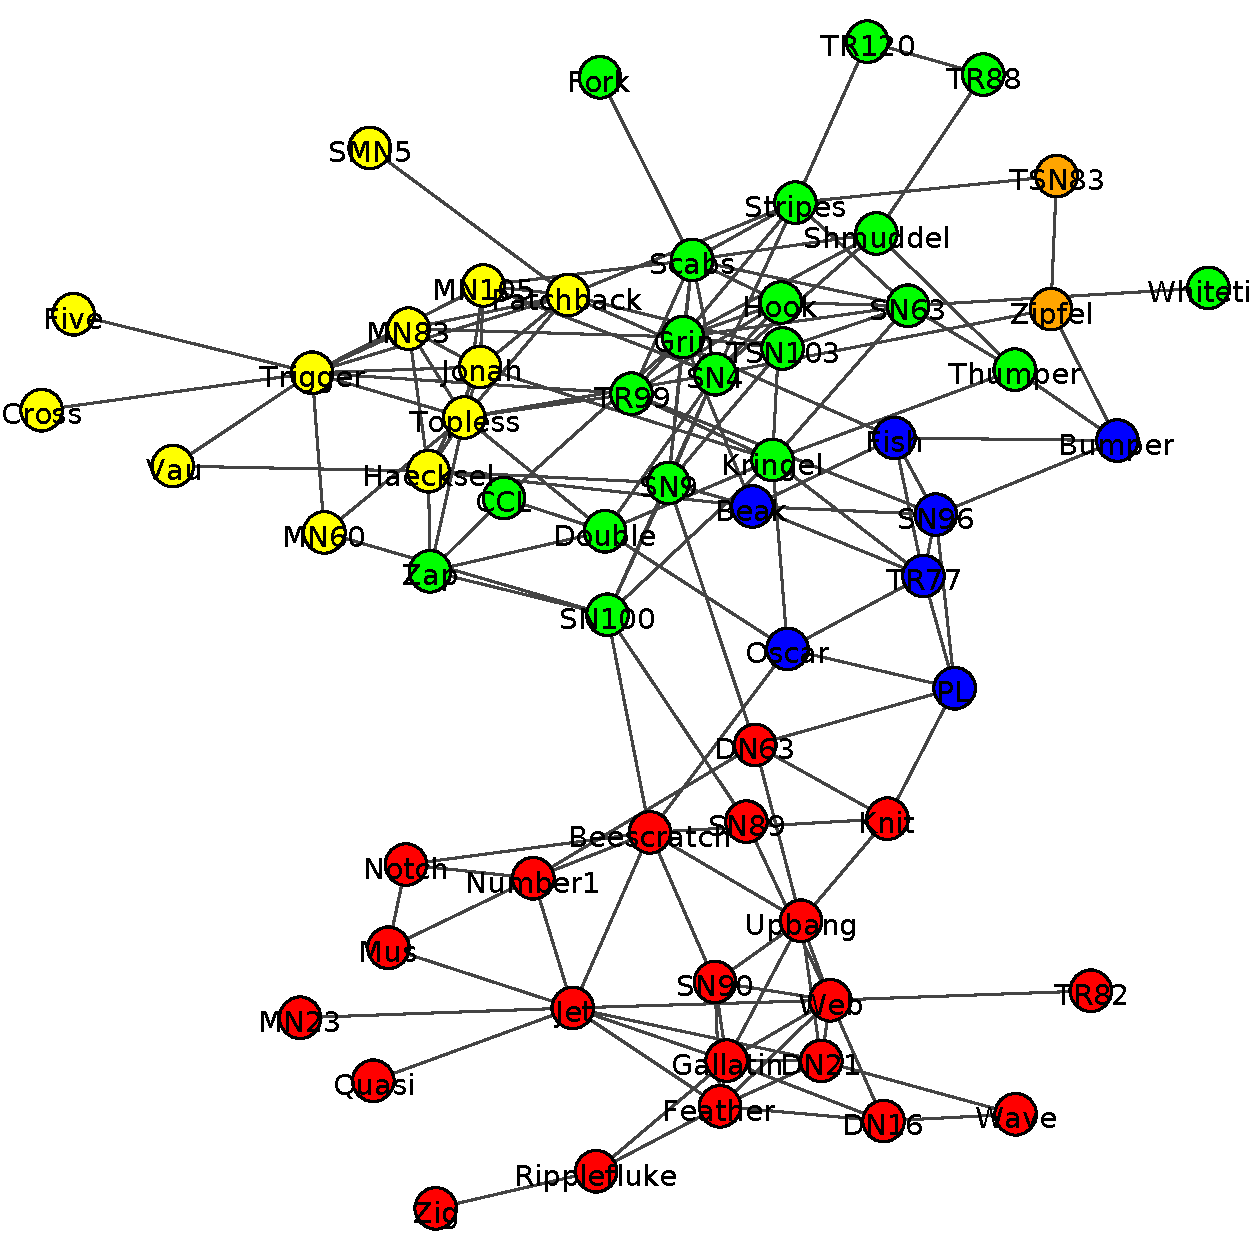
\includegraphics[scale = 0.2]{figuras/Edge_betweenness}
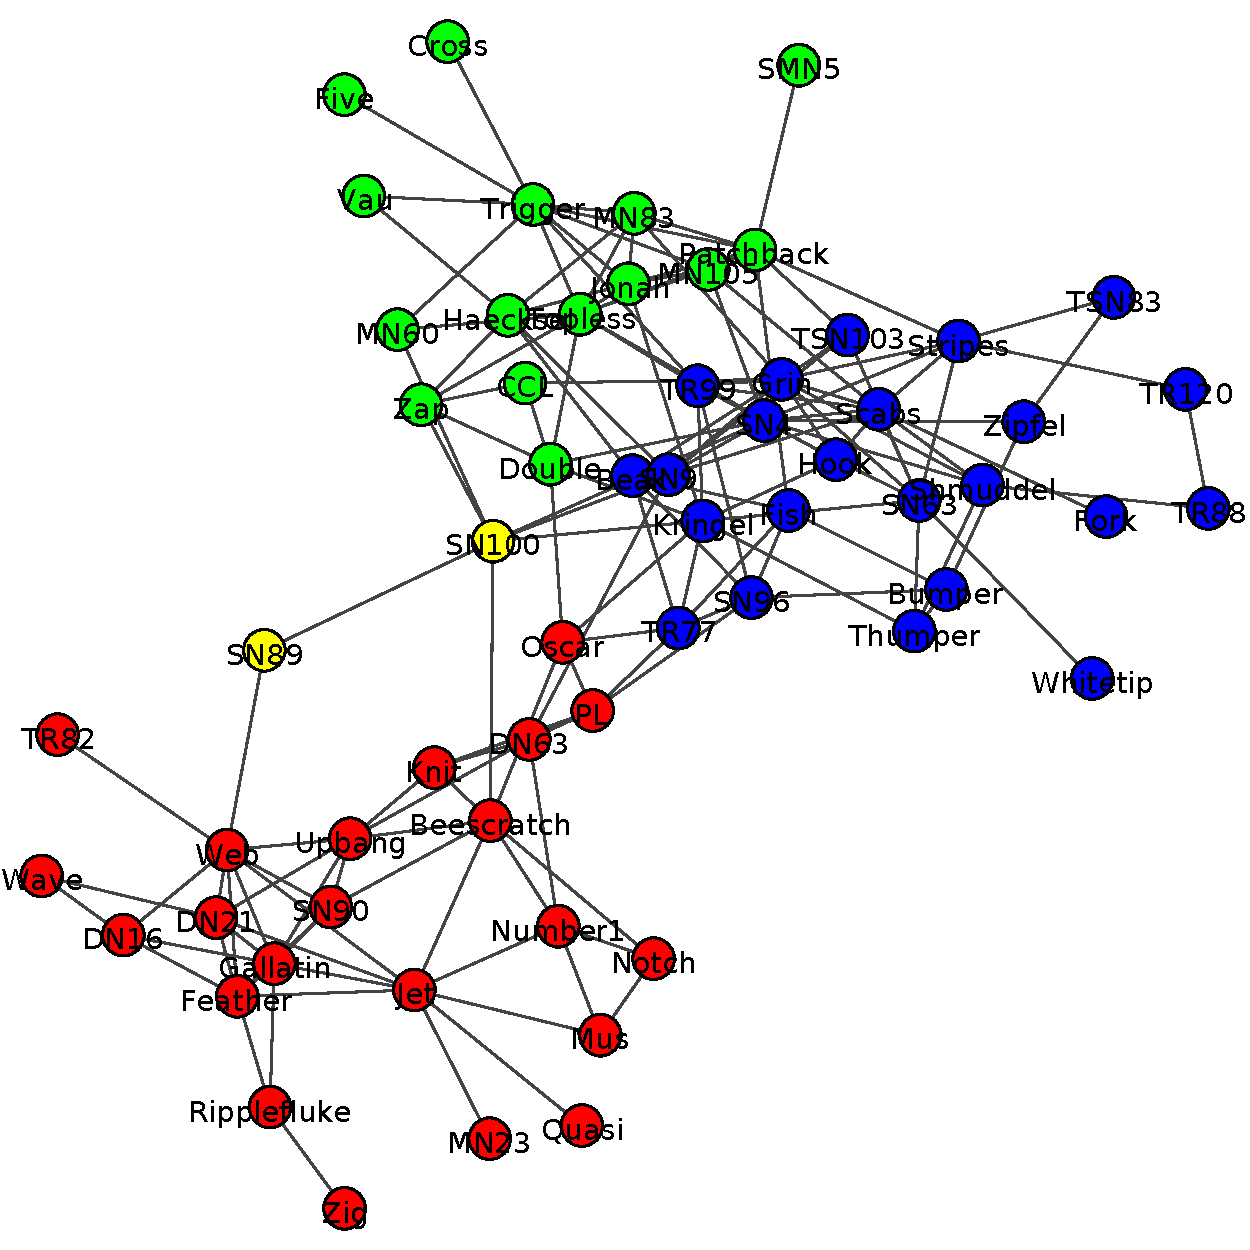
\includegraphics[scale = 0.2]{figuras/Fast_greedy} \\
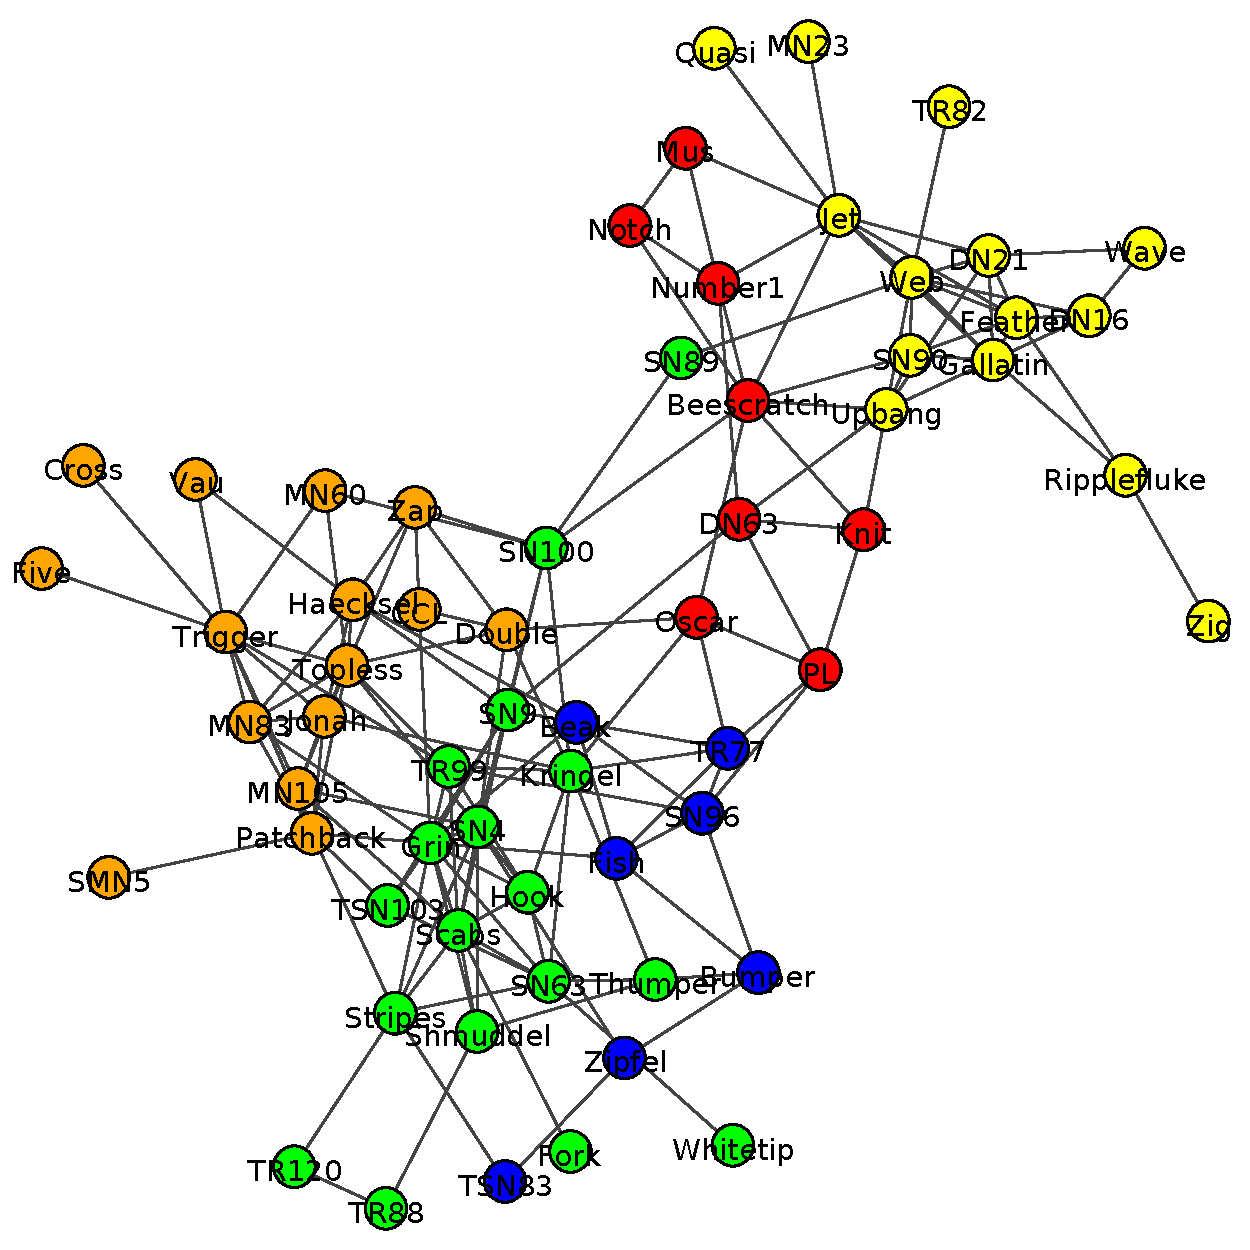
\includegraphics[scale = 0.2]{figuras/Louvain}
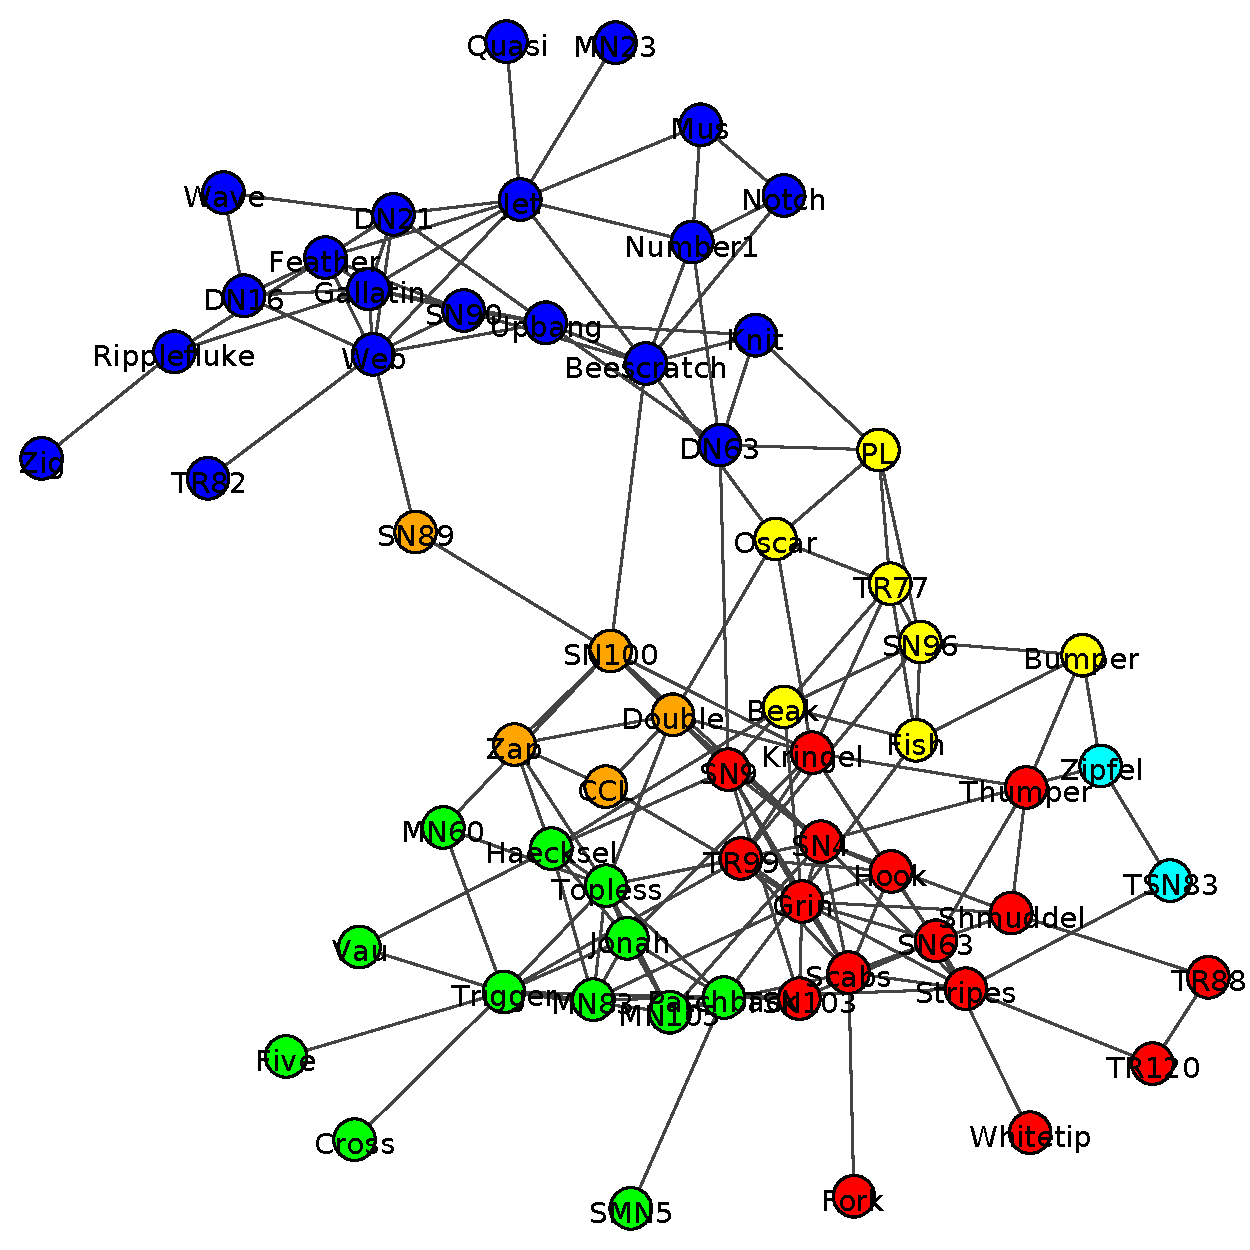
\includegraphics[scale = 0.2]{figuras/Infomap}
\caption{Layouts indicando el cluster asignado por cada algoritmo.}
\label{fig:Layouts_clusters}
\end{figure}

\section{Modularidad}

\begin{table}
\centering
\begin{tabular}{c c c}
\hline \hline
Algoritmo & Modularidad & Silhouette \\
\hline
Edge-betweenness & 0.519 & 0.338 \\
Fast greddy & 0.495 & 0.184 \\
Louvain & 0.519 & 0.294 \\
Infomap & 0.529 & 0.328 \\
\hline\hline
\end{tabular}
\caption{Modularidad y Silhouette de las particiones dadas por diferentes algoritmos.}
\label{table:Modularidad}
\end{table}


\begin{figure}
\centering
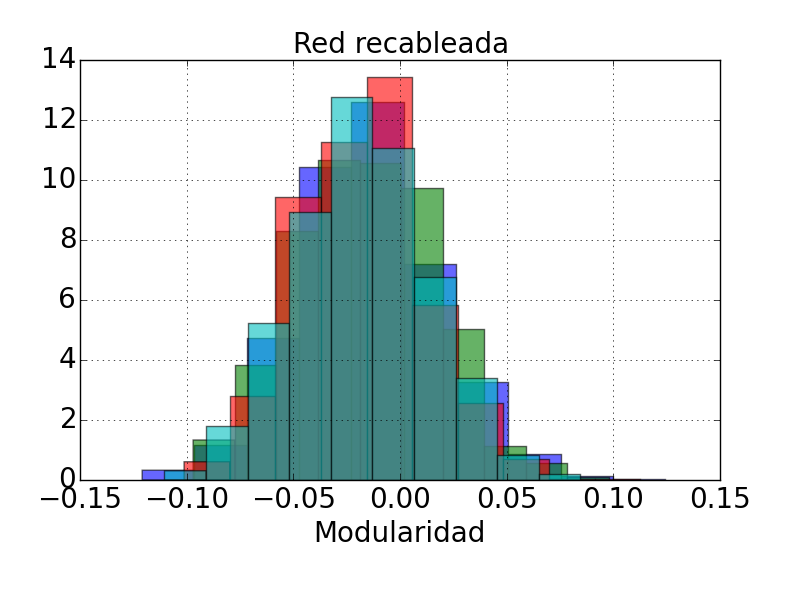
\includegraphics[scale = 0.5]{figuras/Modularidad_random}
\includegraphics[scale = 0.5]{figuras/Silhouette_random}
\caption{Modularidad y Silhouette recableando en forma aleatoria, manteniendo la pertenencia a cada cluster dada por los algoritmos de detección de particiones.Se puede observar que la probabilidad de obtener los valores de la tabla \ref{table:Modularidad} dada una reconexión aleatoria es prácticamente nula.}
\label{fig:Modularidad_random}
\end{figure}

    \input{raul}
    \input{mariela}
    %--- commands/defs
\newcommand{\img}[2]{\includegraphics[scale=#1]{{#2}.png}}
\newcommand{\jmc}[1]{{\color{red}{(JM: #1)}}}   % jimmy comment
\newcommand{\cm}[1]{{\color{blue}{(RB \& MC: #1)}}}   % raul & mari comment



%--- doc
\newpage
\section{Relaci\'on entre comunidades}
\label{sec:info_mutua}

%Para cuantificar la relaci\'on entre el g\'enero de los delfines y la estructura de comunidades que fueron deducidas por los diferentes algoritmos (e.g. {\it Greedy}), empleamos la definici\'on de {\it Informacion Mutua}:
%Para cuantificar la relaci\'on entre comunidades de la red, definidas por dos conjuntos etiquetas de la red, $\{c1\}$ y $\{c2\}$, podemos usar la definici\'on de {\it Informacion Mutua}:
A trav\'es del \'indice de \textit{Informaci\'on Mutua} podemos cuantificar la 
similitud entre particiones, de  comunidades de la red, definidas por dos 
conjuntos etiquetas $\{C_1\}$ y $\{C_2\}$. Este est\'a dado por
\begin{align}
    I(\{C_1\},\{C_2\}) = \sum_{C_1 ,C_2} p(C_1,C_2) \log \frac{p(C_1,C_2)}{p(C_1) p(C_2)},
\label{eq:info_mutua}
\end{align}
o su versi\'on normalizada
\begin{align}
    \label{eq:info_mutua_norm}
    I_n (\{C_1\},\{C_2\}) &= \frac{ 2 I(\{C_1\},\{C_2\}) }{  H(\{C_1\}) + H(\{C_2\}) }  \\
    \intertext{donde}
    H(C) &= - \sum_{c_i \in C} p(c_i) \log(p(c_i))
\end{align}
es la informaci\'on total de la partici\'on $C\equiv \{c_i\}$.



La definici\'on \ref{eq:info_mutua} cuantifica en cuánto coinciden las particiones obtenidas por dos algoritmos diferentes.
%--- valor de In en dos casos extremos
En el caso particular en que los conjuntos $\{C_1\}$ y $\{C_2\}$ estén descorrelacionados, entonces se dice que el conjunto $\{C_1\}$ no brinda ninguna informaci\'on sobre el conjunto $\{C_2\}$, y de acuerdo a la ec. \ref{eq:info_mutua_norm} obtenemos $I_n=0$.
Yi en el caso particular en que $\{C_1\}$ y $\{C_2\}$ son el mismo conjunto, obtenemos la informaci\'on mutua normalizada $I_n=1$, es decir, dos algoritmos diferentes encuentran exactamente la misma comuna.

\subsection{Comparaci\'on entre algoritmos de reconocimiento de comunidades}

La cuantificaci\'on de {informaci\'on dada por la Ec. \ref{eq:info_mutua} 
consta tanto de: la medici\'on de la probabilidad de que un nodo pertenezca
a una comunidad $C_i$ ($p(C_i)$), como de la probabilidad conjunta de que un
nodo pertenezca a una comunidad $C_i$ en la partici\'on $\{C_i\}$ y pertenezca
a la comunidad $C_j$ en la partici\'on $\{C_j\}$ ($p(C_i,C_j)$). La primera
distribuc\'on de pertenencia a etiquetas/comunidades se puede ver en la 
figura \ref{fig:histos}. En ella se puede observar que el etiquetado muestra 
distintas distribuciones en cada caso, adem\'as es importante notar que 
etiquetados iguales no representan las mismas comunidades entre cada algoritmo,
por lo tanto, no existe una \'unica distribuci\'on que represente cada caso;
Por otro lado, el caso de la probabilidad
conjunta es mostrado en las matrices de la figura \ref{fig:matrix}.


\begin{figure}[!ht]
    \centering
    \begin{subfigure}[b]{.45\columnwidth}
        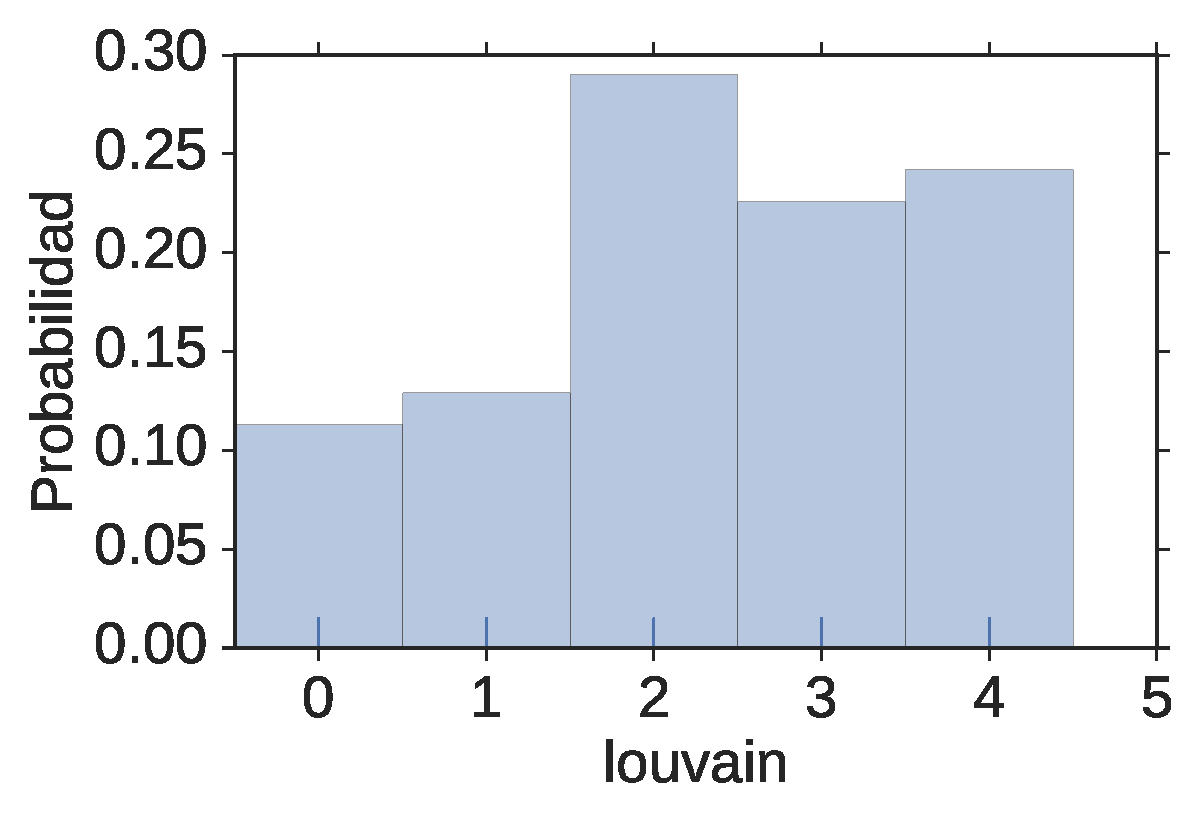
\includegraphics[width=0.95\columnwidth]{figuras/louvain_probability.pdf}
    \end{subfigure}
    \begin{subfigure}[b]{.45\columnwidth}
        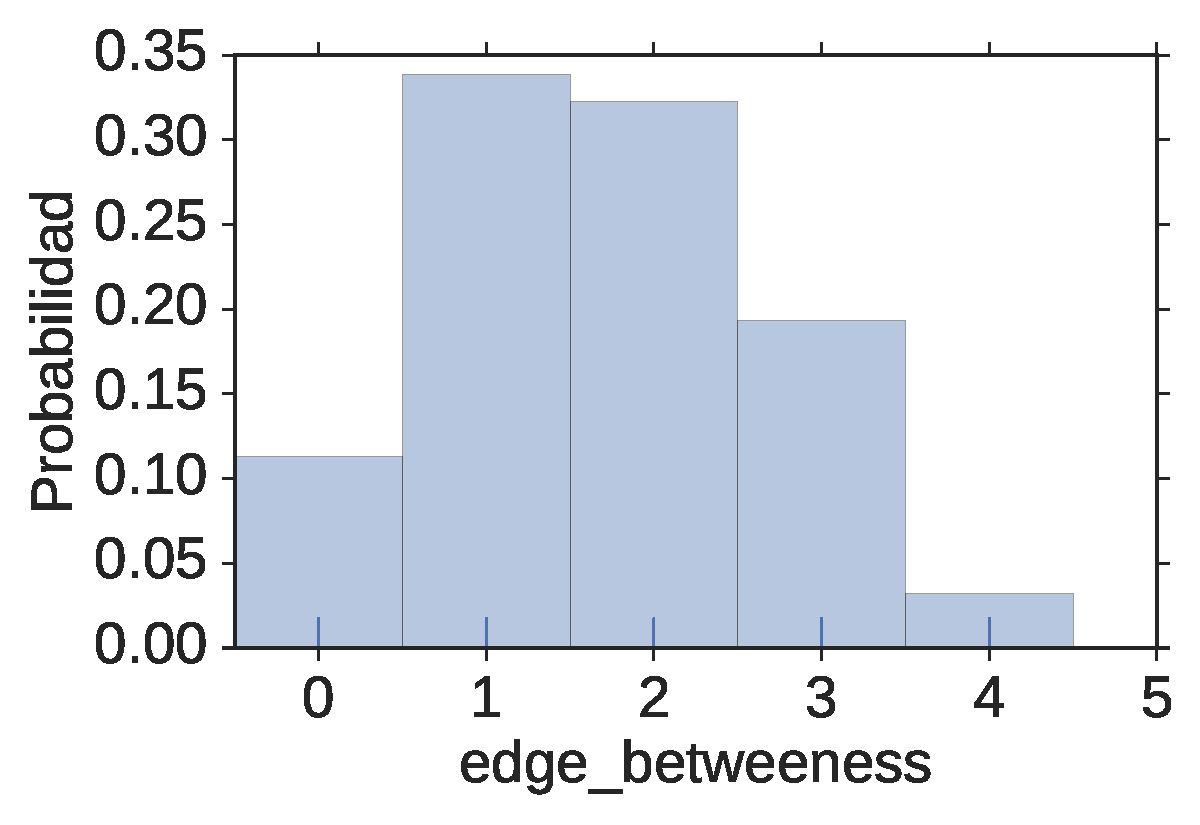
\includegraphics[width=0.95\columnwidth]{figuras/edge_betweeness_probability.pdf}
    \end{subfigure}\\
    \begin{subfigure}[b]{.45\columnwidth}
        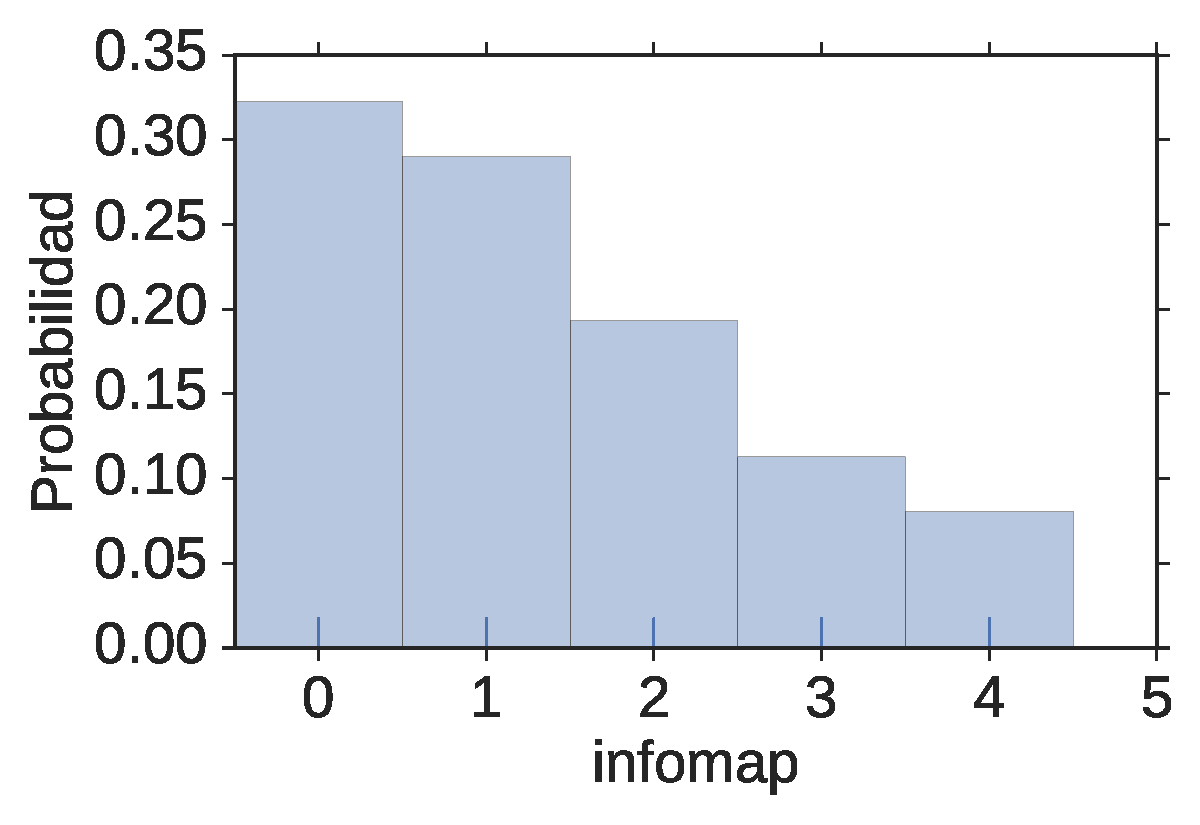
\includegraphics[width=0.95\columnwidth]{figuras/infomap_probability.pdf}
    \end{subfigure}
    \begin{subfigure}[b]{.45\columnwidth}
        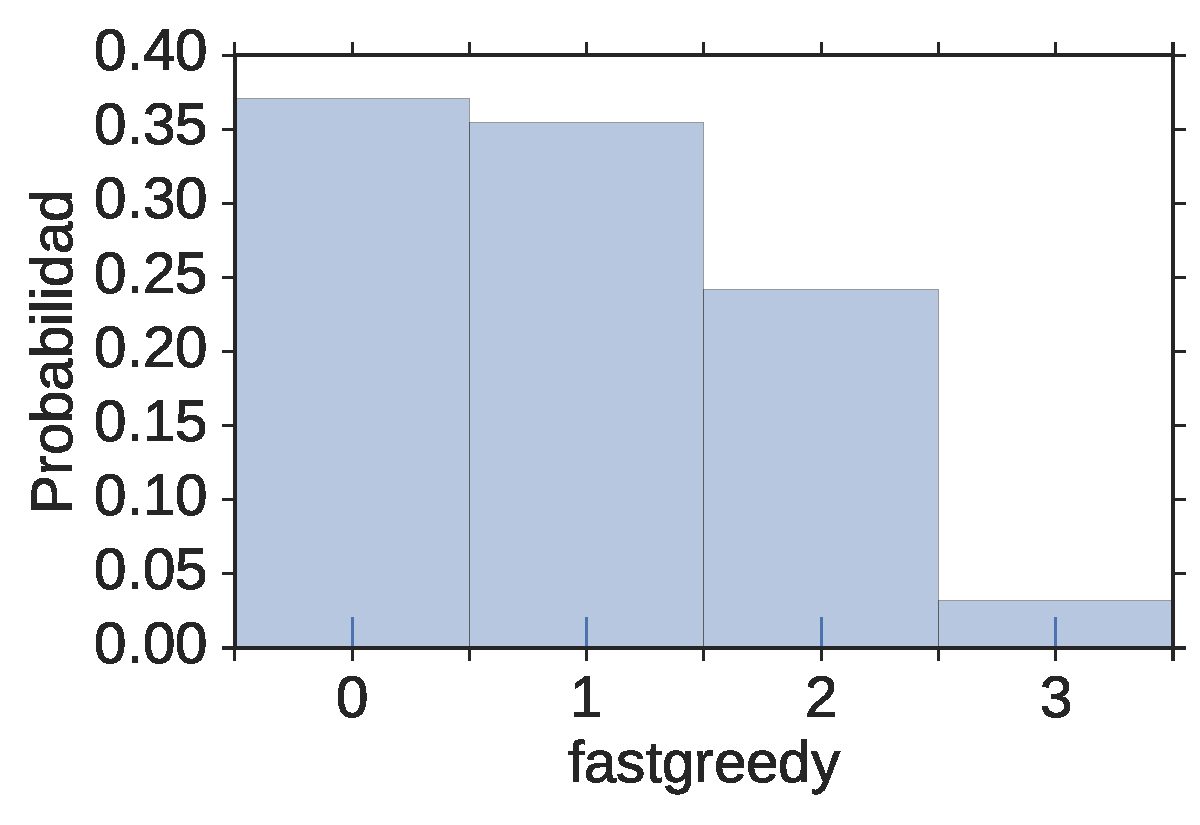
\includegraphics[width=0.95\columnwidth]{figuras/fastgreedy_probability.pdf}
    \end{subfigure}
    \caption{\label{fig:histos} Distribuci\'on de probabilidad de pertenencia de un nodo a una comunidad 
para los diferentes algoritmos utilizados.}
\end{figure}




\begin{figure}[!ht]
    \centering
    \begin{subfigure}[b]{.45\columnwidth}
        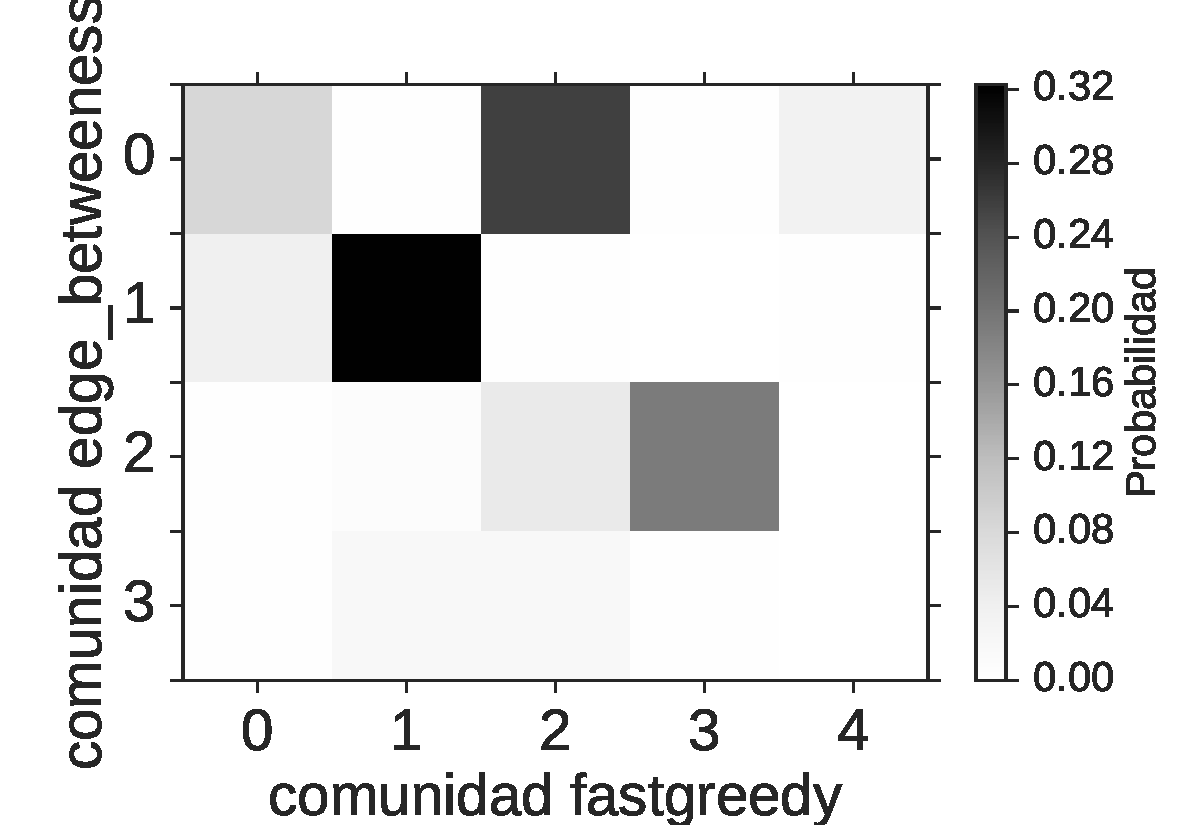
\includegraphics[width=0.95\columnwidth]{figuras/join_proba_fastgreedy-edge_betweeness.pdf}
    \end{subfigure}
    \begin{subfigure}[b]{.45\columnwidth}
        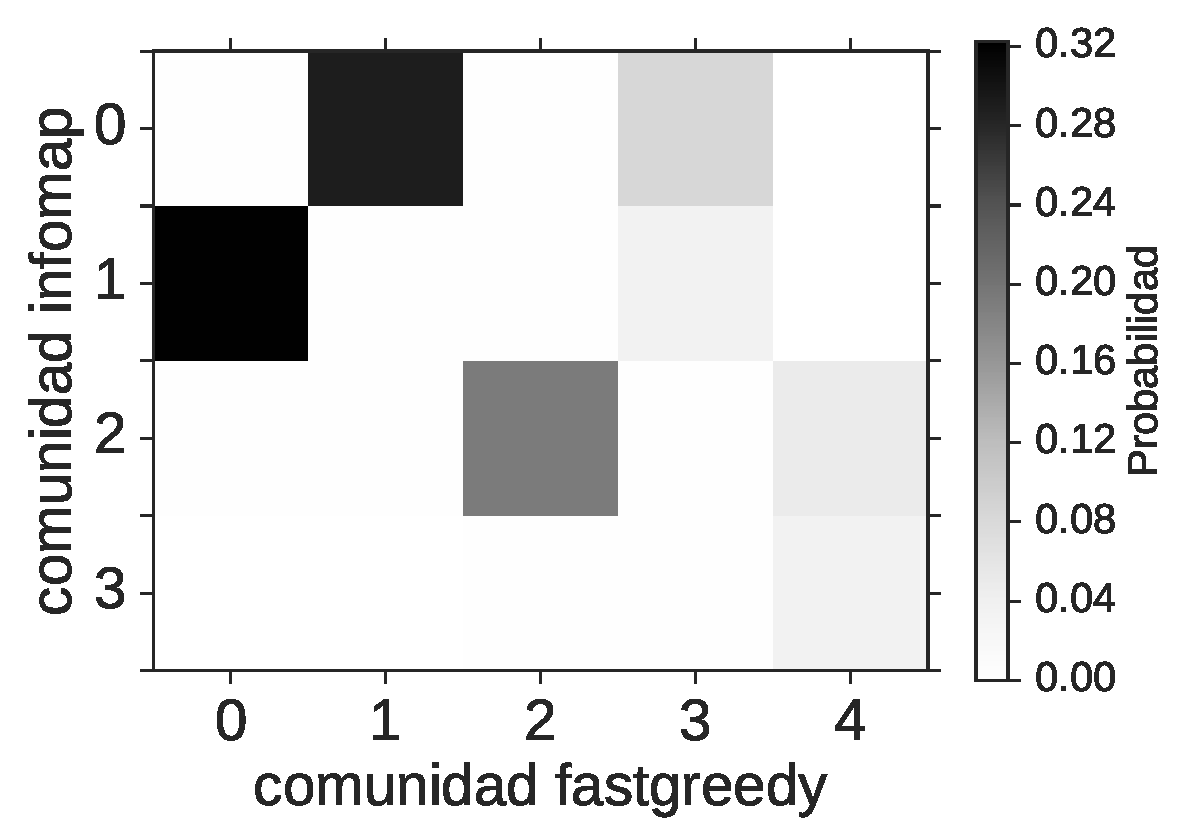
\includegraphics[width=0.95\columnwidth]{figuras/join_proba_fastgreedy-infomap.pdf}
    \end{subfigure}\\
    \begin{subfigure}[b]{.45\columnwidth}
        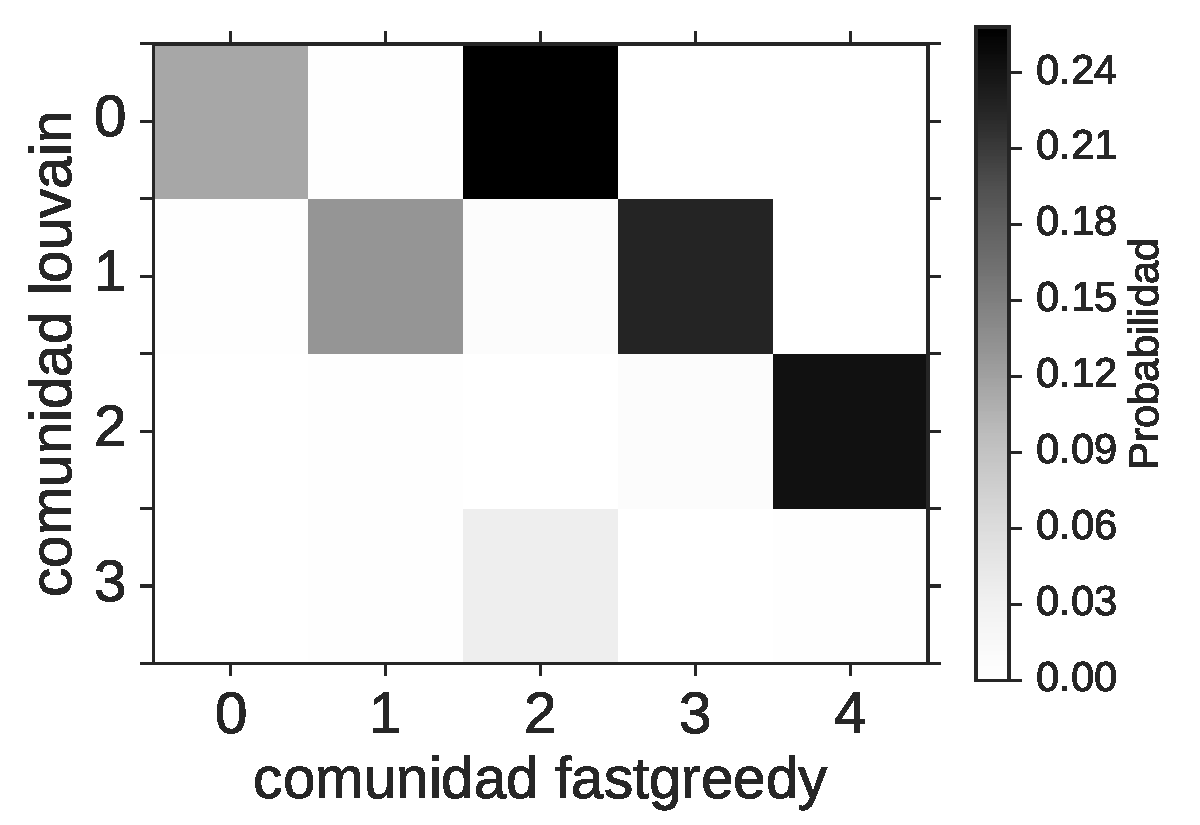
\includegraphics[width=0.95\columnwidth]{figuras/join_proba_fastgreedy-louvain.pdf}
    \end{subfigure}
    \begin{subfigure}[b]{.45\columnwidth}
        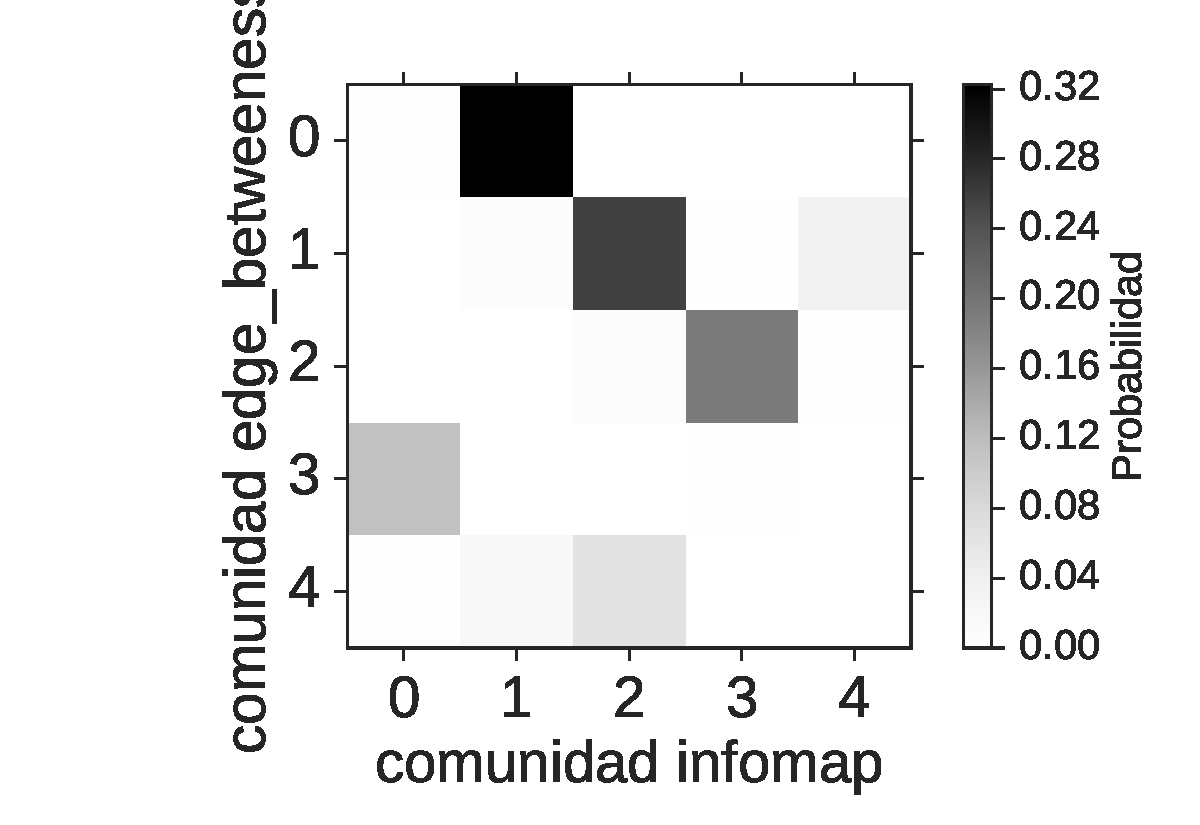
\includegraphics[width=0.95\columnwidth]{figuras/join_proba_infomap-edge_betweeness.pdf}
    \end{subfigure}\\
    \begin{subfigure}[b]{.45\columnwidth}
        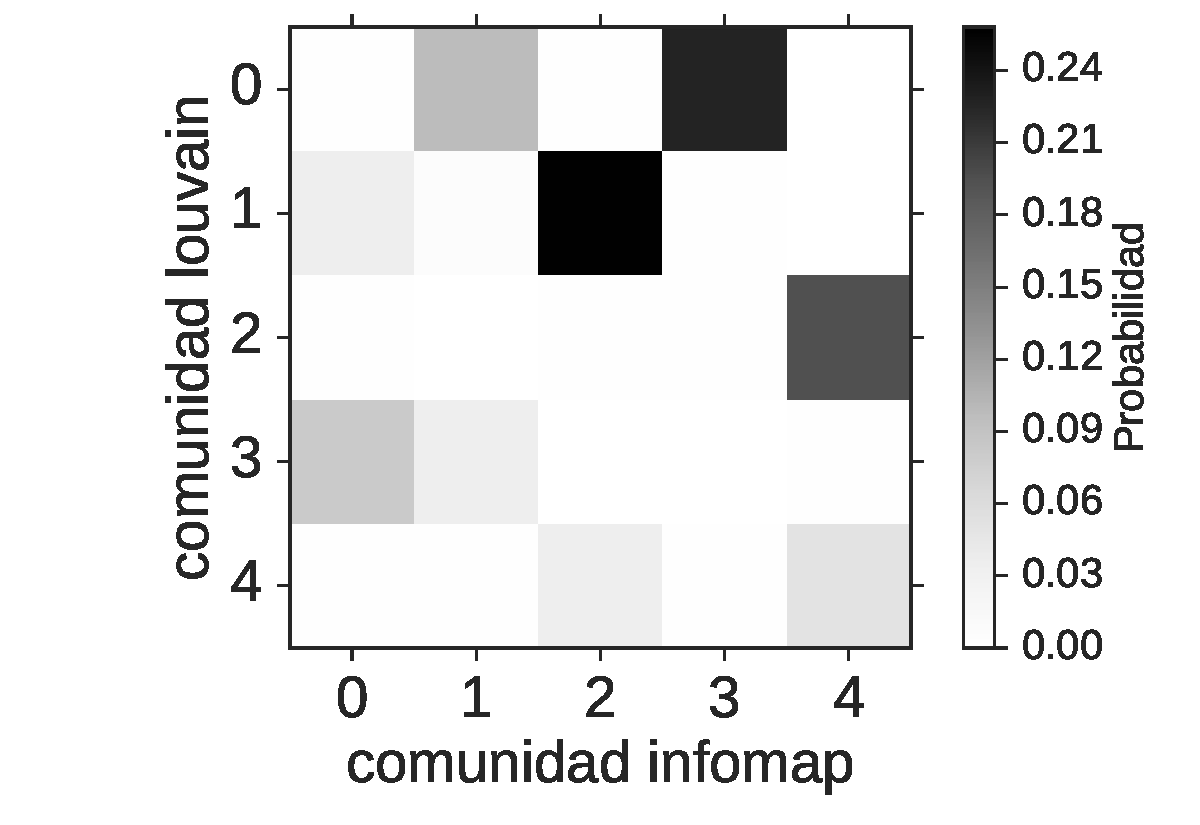
\includegraphics[width=0.95\columnwidth]{figuras/join_proba_infomap-louvain.pdf}
    \end{subfigure}
    \begin{subfigure}[b]{.45\columnwidth}
        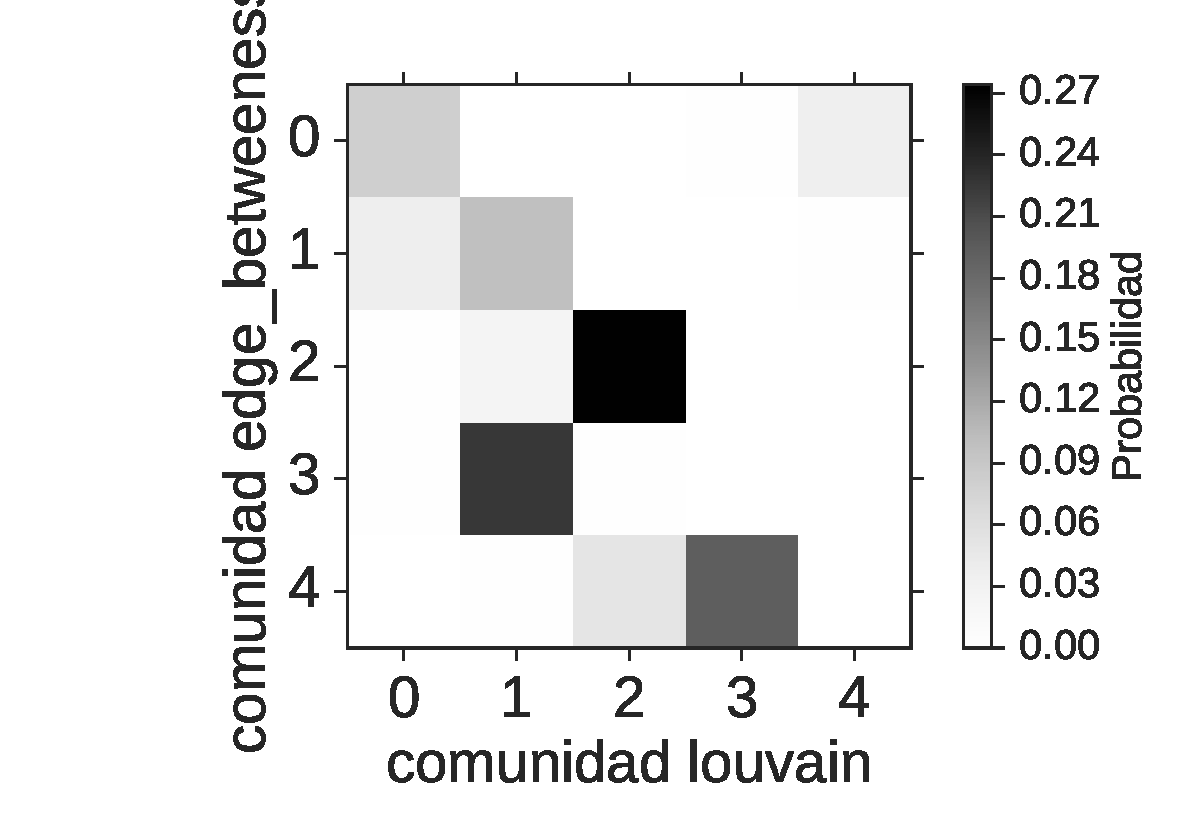
\includegraphics[width=0.95\columnwidth]{figuras/join_proba_louvain-edge_betweeness.pdf}
    \end{subfigure}
    \caption{\label{fig:matrix} Distribuci\'on de probabilidad conjunta de pertenencia de un nodo a una comunidad 
de cada par de algotirmos.}
\end{figure}

El valor medio (de 1000 iteraciones) de la \textit{Informaci\'on Mutua} total, normalizada, 
es mostrada en la 
Tabla \ref{tab:mi} de la cual se puede observar que los algoritmos {\it infomap}
y {\it Edge Betweeness} son los m\'as similares con una semejanza del $86.1\%$,  
las rutinas {\it Fast Greedy} y {\it Edge Betweeness} muestran la menor correlaci\'on
con una similitud del $66.2\%$ mientras que en general el resto coinciden en un rango 
de $70\%-80\%$


\begin{table}[!h]
    \centering
    \caption{\label{tab:mi} Informaci\'on mutua entre las particiones encontradas por cada algoritmo.}
    {\scriptsize
    \begin{tabularx}{0.9\textwidth}{Xl|ccccX}
        \hline\hline
        &                 &  Fast Greedy    & Edge betweeness   & Infomap   & Louvain &  \\
        \hline
        & Fast Greedy     & 1.000           & 0.662             & 0.782     & 0.794 \\
        & Edge Betweeness &                 & 1.000             & 0.861     & 0.732 \\
        & Infomap         &                 &                   & 1.000     & 0.783 \\
        & Louvain         &                 &                   &           & 1.000 \\
        \hline\hline
    \end{tabularx}
    }
\end{table}




\newpage
\subsection{Relaci\'on de las comunas con g\'enero}
\label{sec:relacion_con_genero}

Para cuantificar la relaci\'on entre las comunas deducidas por los diferentes algoritmos (e.g. {\it greedy}) y el g\'enero, usamos la ec. \ref{eq:info_mutua_norm} identificando a las comunas con $\{C_1\}$ y a las etiquetas de g\'enero con $\{C_2\}$.
%--- ahora veamos nuestro caso
En la figura \ref{fig:prob_conj} mostramos, en el encabezado de cada panel, los valores de la informaci\'on mutua $I_n$, los cuales caen en el intervalo $(0.10 - 0.21)$, es decir que $I_n \ll 1$ en todos los casos; esto nos dice que el conjunto de comunas ($\{C_1\}$) deducido por cierto algoritmo (e.g. {\it greedy}) no nos da mucha informaci\'on sobre el g\'enero ($\{C_2\}$).
%--- test de consistencia
Como test de consistencia para esto  \'ultimo, hicimos sorteos del g\'enero de cada nodo(manteniendo constante el n\'umero total de masculinos y femeninos por separado), y contabilizamos el n\'umero de enlaces entre pares de g\'eneros distintos $n_ig$.
En la figura \ref{fig:hist_sort_sex} mostramos un histograma de $n_ig$, y en l\'inea negra el valor asociado para la red real (original).
De aqui vemos que el valor de la red real esta apartado $\sim 1 \sigma$ del valor medio del histograma; lo cual significa que hay una ligera tendencia a que las comunas tengan muchos ejemplares de un sexo en particular. 
Esto \'ultimo es consistente con el bajo valor de $I_n$ discutido mas arriba.
Sin embargo, la diferencia no parece ser significativa: la probabilidad de obtener el valor actual de número de links entre delfines de distinto género y misma comuna, dada una distribución de sexos al azar, es de aproximadamente 5\%, por lo tanto no es tan improbable obtener este valor en una asignación aleatoria de géneros.



%--- prob conjunta `p12` para c/algoritmo
\begin{figure}
    \centering
    \img{0.5}{p12_greedy}
    \img{0.5}{p12_betweenness}
    \img{0.5}{p12_infomap}
    \img{0.5}{p12_louvain}
    \caption{
    Valores de las matrices de probabilidad conjunta para los algoritmos {\it greedy} (izquierda, arriba) {\it betweenness} (derecha, arriba), {\it infomap} (izquierda, abajo) y {\it louvain} (derecha, abajo). 
    }
\label{fig:prob_conj}
\end{figure}


%--- histograma de sorteos de sexo
\begin{figure}
    \centering
    \img{0.6}{hist_sort_sex}
    \caption{
    Distribuci\'on del n\'umero de enlaces entre g\'eneros diferentes, para diferentes realizaciones de sorteo del sexo de los nodos de la red (manteniendo constante el n\'umero de masculinos y femeninos por separado).
    La l\'inea negra muestra el valor que corresponde a la red original que caracterizamos en este trabajo.
    La zona sombreada en celeste representa la regi\'on que cubre la desviaci\'on est\'andar respecto de la media.
    El valor de la red original (o real) se aparta $\sim 1 \sigma$ respecto del centro de la distribuci\'on, lo cual muestra una ligera tendencia a la existencia de comunas que tienen muchos ejemplares de un sexo en particular.
    Esto es consistente con el bajo valor ($\ll 1$) de la informaci\'on mutua $I_n$ (ver ec. \ref{eq:info_mutua_norm} y Secc. \ref{sec:info_mutua}).
    }
\label{fig:hist_sort_sex}
\end{figure}

%EOF


%\bibliographystyle{plainnat}
%\bibliography{biblio}

\end{document}
